%%%%%%%%%%%%%%%%%%%%%%%%%%%%%%%%%%%%%%%%%%%%%%%%%%%%%%%%%%%%%%%
% sample chapter
%
% Copy it to a new file with a new name and use it
% use it as a template for your own input.
%
%%%%%%%%%%%%%%%%%%%%%%%% Springer-Verlag %%%%%%%%%%%%%%%%%%%%%%%%%%

\chapter{Appendix Heading}
\label{A:app} % Give a unique label

Your text comes here. Separate text sections

\section{Section Heading}
\label{A:sec:1}  % Give a unique label
%and use \ref{sec:1} and \cite{journal1}

\subsection{Subsection Heading}
\label{A:sec:2}

\subsubsection{Subsubsection Heading}

\paragraph{Paragraph Heading}
\subparagraph{Subparagraph Heading.} as required%
\index{paragraph}. % Use the \index command for coding your index

% For tables use
%
\begin{table}
\centering
\caption{Please write your table caption here}
\label{A:tab:1}       % Give a unique label
% For LaTeX tables use
\begin{tabular}{lll}
\hline\noalign{\smallskip}
first & second & third  \\
\noalign{\smallskip}\hline\noalign{\smallskip}
number & number & number \\
number & number & number \\
\noalign{\smallskip}\hline
\end{tabular}
\end{table}
%
%
% For figures use
%
\begin{figure}
\centering
% Use the relevant command for your figure-insertion program
% to insert the figure file.
% For example, with the option graphics use
\includegraphics[height=3cm]{figure.eps}
% If not, use
%\picplace{5cm}{2cm} % Give the correct figure height and width in cm
\caption{Please write your figure caption here}
\label{A:fig:1}       % Give a unique label
\end{figure}


